% Guard: macros.tex is \input both by main.tex (after the packages it needs,
% e.g. amsmath for \DeclareMathOperator) and by individual section files so
% they remain compilable on their own. Loading it twice would redefine every
% \newcommand and abort, so the second and later loads are no-ops.
\ifdefined\PQRmacrosloaded\endinput\fi
\let\PQRmacrosloaded\relax

% --- 0. revision marking ---
% Text added to Section 2 during the current revision is wrapped in \added{...}
% so the advisors can see at a glance what is new. Redefine to \relax to print
% the paper without the marking.
\newcommand{\added}[1]{\textcolor{blue}{#1}}
\long\def\added#1{\begingroup\color{blue}#1\endgroup}  % \long: may span paragraphs


% --- A. operator-style score and function names ---
\newcommand{\HD}{\mathit{HD}}                        % histogram distance; use \HD_\gamma
\newcommand{\Attr}{\mathit{Attr}}                    % attribute set of a schema
\newcommand{\Attrs}{\mathit{Attrs}}                  % attribute set argument
% Abbreviated in MATH only; the prose still spells the names out in full.
% Spelling them out inside formulas makes displayed equations far too wide
% for a two-column layout (the product-rule step below overflowed by 200pt).
\newcommand{\Use}{\mathit{Use}}
\newcommand{\Cov}{\mathit{Cov}}
\newcommand{\Rep}{\mathit{Rep}}
\newcommand{\DivS}{\mathit{Div}}
\newcommand{\TVD}{\mathit{TVD}}
\newcommand{\GS}{\mathit{GS}}                        % global sensitivity
\DeclareMathOperator{\Dom}{Dom}
\DeclareMathOperator{\Lap}{Laplace}

% --- B. core objects ---
\newcommand{\Qone}{Q_1}
\newcommand{\Qtwo}{Q_2}
\newcommand{\pD}{p(D)}
\newcommand{\views}{\mathcal{P}}
\newcommand{\hist}[2]{H_{#1,#2}}                     % \hist{\Qone(\pD)}{A}
\newcommand{\dhist}{\Delta H}
\newcommand{\nhist}{\widetilde{\Delta H}}            % the released noisy object

% --- C. privacy budget and parameters ---
\newcommand{\eps}{\epsilon}
\newcommand{\epsP}{\epsilon_P}
\newcommand{\epsS}{\epsilon_S}
\newcommand{\epsH}{\epsilon_H}
\newcommand{\gammaref}{\gamma_{\mathrm{ref}}}
\newcommand{\gammaeval}{\gamma_{\mathrm{eval}}}
\newcommand{\taumax}{\tau_{\max}}

% --- D. mechanisms ---
\newcommand{\ExpMech}{\textsc{ExpMech}}
\newcommand{\OneShotTop}[1]{\textsc{OneShotTop-}#1}
\newcommand{\AdaptiveTau}{\textsc{AdaptiveTau}}
% --- E. experiment baselines (used in sections/experiments.tex) ---
\newcommand{\Bone}{\ensuremath{\mathsf{B1}}}
\newcommand{\Btwo}{\ensuremath{\mathsf{B2}}}
\newcommand{\Bthree}{\ensuremath{\mathsf{B3}}}

\section{Problem Statement and Model}\label{sec:model}

This section states what an explanation is and what we are looking for (Section~\ref{subsec:private-query-difference-setting}), gives the measures of explanation quality as modifications of the forms used in prior work (Section~\ref{sec:explanation-quality}), bounds the sensitivity of each of them (Section~\ref{subsec:ideal-sensitivity}), and derives from that the two-stage structure the framework uses and the two utilities it optimises (Section~\ref{subsec:two-stages}).

\subsection{Private Explanations of Query Differences}
\label{subsec:private-query-difference-setting}

We consider a trusted server that holds a private database $D$ and two related queries $Q_1$ and $Q_2$ over it.
The second query is typically derived from the first by a mechanism that the framework treats as a black box.
In query refinement (Definition~\ref{def:refinement}), $Q_1=Q$ is the original query and $Q_2=Q'$ its refinement; in consistent query answering (Definition~\ref{def:consistent-answer}), $Q_2$ is $Q_1$ evaluated under repair semantics.
Both are instances of the same problem, explaining how two related queries differ on the same database, and the framework does not depend on which one produced the pair.
For a view $p$ we write $Q_i(p(D))$ for the restriction of the output of $Q_i$ to the view, $Q_i(D)\cap p(D)$ (Section~\ref{subsec:prelim-settings}); for a selection query it is the result of evaluating $Q_i$ on $p(D)$ (Proposition~\ref{prop:view-restriction}).

\emph{Our goal} is to let an analyst see \emph{how} the two outputs differ - which parts of the population the change added, removed or reshaped - while revealing nothing about any individual in $D$.
Two things have to be settled for that: what an explanation looks like, and what makes one good.
This subsection settles the first, and Section~\ref{sec:explanation-quality} the second; given those quality measures, the task is to return a handful of explanations that score well under them, privately.

\paragraph{Workflow.}
An analyst submits a query $Q_1$ to the server; the server obtains $Q_2$, either because the analyst supplies it or because an external mechanism - a refinement algorithm, a repair procedure -- derives it (Figure~\ref{fig:framework}).
The server evaluates both, privately selects a small set of predicate views and, within them, the explanation candidates that best characterise the difference, and finally releases noisy histograms for the selected candidates.
Only this last object leaves the server; the analyst never observes $D$, the exact outputs, or the exact scores that drove the selection.
The mechanism producing $Q_2$ is outside the scope of the privacy analysis, which accounts only for the explanation.
\alon{Done: trusted-server workflow described above and depicted in Figure~\ref{fig:framework}.}

\begin{figure*}[t]
\centering
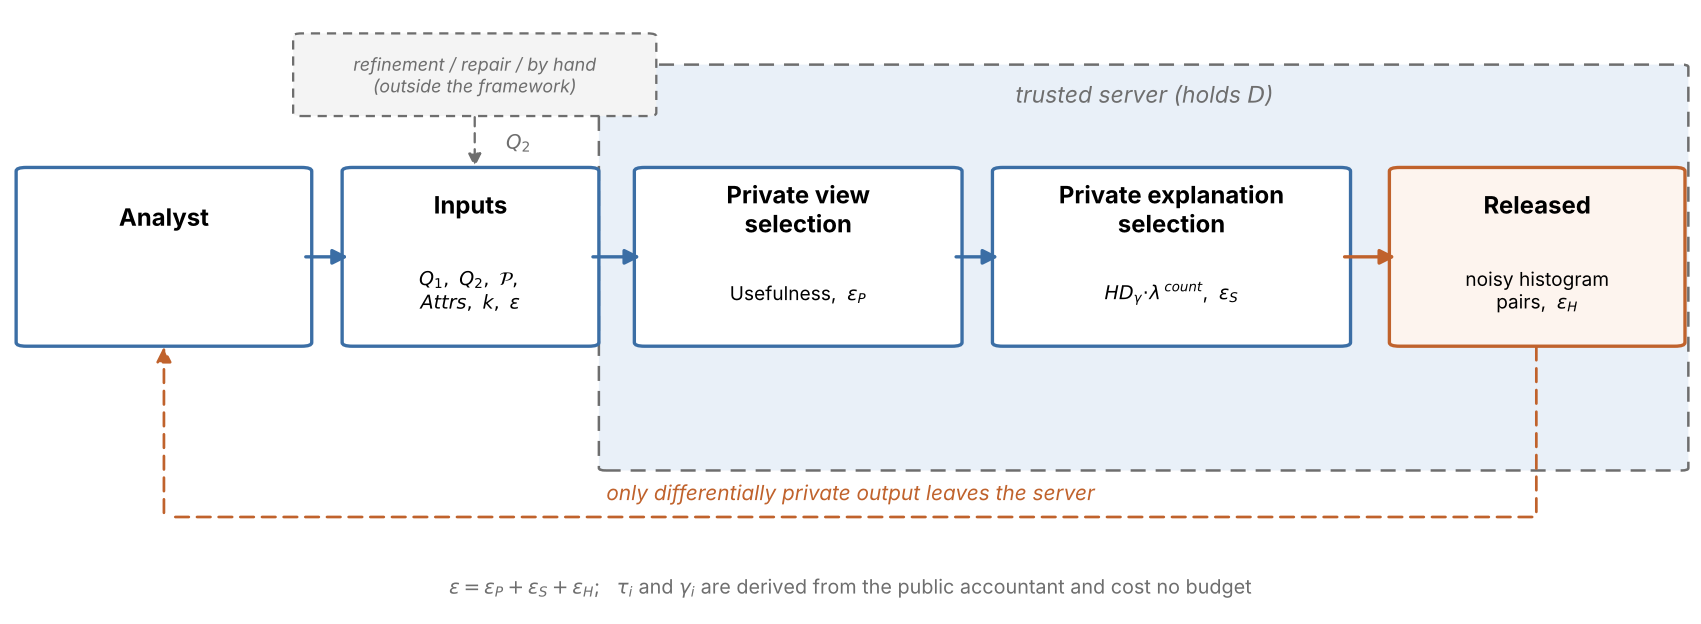
\includegraphics[width=\linewidth]{figures/framework.png}
\caption{The private query-difference explanation framework.
The analyst submits $Q_1$; the related query $Q_2$ is produced by a black-box refinement or repair mechanism.
The server privately selects views, then explanations, and releases only noisy histograms.
The per-round parameters $\tau_i$ and $\gamma_i$ are functions of the public privacy accountant and therefore consume no budget.}
\label{fig:framework}
\end{figure*}

\paragraph{The structure of an explanation.}
An explanation answers \emph{where} the two outputs differ and \emph{in what respect}.
The where is a region of the database, given by a view predicate $p\in\views$; the respect is an attribute $A\in\Attrs$, whose distribution the two outputs are compared on.

\begin{definition}[Histogram Explanation Candidate]
\label{def:candidate}
Given a view $p\in\views$ and an explanation attribute $A\in\Attrs$, the \emph{histogram explanation candidate} $e=(p,A)$ induces the two histograms
\[
    \hist{Q_1(\pD)}{A}
    \qquad\text{and}\qquad
    \hist{Q_2(\pD)}{A}.
\]
We write $\mathcal{C}=\views\times\Attrs$ for the space of candidates, and $E\subseteq\mathcal{C}$ for a set of them.
\end{definition}

What is released for a selected candidate is a perturbed version of its two histograms, in the sense of the Laplace mechanism (Definition~\ref{def:laplace-mechanism}).

\begin{definition}[Noisy histogram]
\label{def:noisy-histogram}
For a set of tuples $T\subseteq D$, an attribute $A$ and a scale $b>0$, the \emph{noisy histogram} of $A$ over $T$ is
\[
\hat H_{T,A}(v)=\hist{T}{A}(v)+Y_v,\qquad v\in\Dom(D[A]),
\]
with $Y_v$ drawn independently from the Laplace distribution of scale $b$, one draw per bin of the public domain of $A$.
\end{definition}

An explanation releases the pair $\big(\hat H_{Q_1(p(D)),A},\hat H_{Q_2(p(D)),A}\big)$.
The analyst reads the two profiles side by side, which is how the change becomes legible: in Example~\ref{ex:candidate} the pair shows $357$ against $1{,}203$ on \texttt{Prof-specialty}, whereas the difference alone, $-846$, reports the size of the shift without the levels that make it interpretable.
The pair is not the cheapest option.
A tuple selected by both queries changes both histograms, so the pair has $L_1$-sensitivity $2$, whereas their difference $\Delta H_{p,A}$ has sensitivity $1$ (Proposition~\ref{prop:histogram-release-sensitivity}): under a fixed budget, releasing a single noisy difference histogram halves the noise scale.
Where budget is scarce the framework can release that difference instead, trading the levels for accuracy.

\alon{Done: a noisy histogram is now defined (Definition~\ref{def:noisy-histogram}), and the released object is the \emph{pair}, which is what the analyst reads; the single difference histogram is kept as the budget-saving variant.}

So an explanation is a region, an attribute, and a pair of noisy histograms over that attribute inside that region.
An answer to the analyst is a small set of these.

\begin{example}[Two explanations of the running refinement]
\label{ex:candidate}
Continuing Example~\ref{ex:running}, where $Q_1$ selects Bachelor's and Master's degree holders working at least $50$ hours and $Q_2$ selects Master's degree holders working at least $30$, take the view $p=(\texttt{education}=\texttt{Masters})$ and the attribute $A=\texttt{occupation}$.
The view holds $2{,}657$ tuples, of which $Q_1$ selects $874$ and $Q_2$ selects $2{,}453$.
The two occupational profiles differ most on \texttt{Prof-specialty} ($357$ against $1{,}203$) and \texttt{Exec-managerial} ($357$ against $757$): inside the Master's population, the refinement does not merely add people, it shifts the occupational mix towards professional-specialty roles.
The explanation released for this candidate is the difference of these two histograms with Laplace noise added per bin.

Now take $p'=(\texttt{education}=\texttt{Bachelors})$.
Here $Q_2(p'(D))=\emptyset$, because $\varphi_2$ requires a Master's degree, while $Q_1(p'(D))$ holds $2{,}181$ of the view's $8{,}025$ tuples, led by \texttt{Exec-managerial} ($736$) and \texttt{Prof-specialty} ($530$).
This candidate reports a population the refinement removes in its entirety --- the kind of change that is invisible in the aggregate value and that a good explanation should surface.
\end{example}

\subsection{Measures of Explanation Quality}
\label{sec:explanation-quality}

The criteria we optimise are the four reviewed in Section~\ref{subsec:prelim-quality}: interestingness, representativeness, coverage and diversity.
None is new.
What is new is the form we give them, and the reason for the change is always the same: a measure whose value can be swung by one individual cannot be optimised under differential privacy at all, because the noise a private mechanism must add is calibrated to exactly that swing.
For each criterion we therefore recall the form used in prior work, say what goes wrong with it here, and give the form we use.
Section~\ref{subsec:ideal-sensitivity} states the effect of all four changes in one place.

\paragraph{Interestingness.}
In its distributional form a candidate is scored by the distance between the two distributions it induces~\cite{SeeDB,FEDEX}, which in our setting is the total variation distance between the conditional distributions of $A$ over $Q_1(p(D))$ and $Q_2(p(D))$, or twice it in the normalised form.
Two things go wrong.
It is undefined when one of the two outputs does not meet the view --- exactly the one-sided views of Example~\ref{ex:candidate}, which report a population a refinement adds or removes wholesale --- and, being a ratio over the output sizes, a single tuple can move it across its entire range (Proposition~\ref{prop:sensitivity-itemized}).
We therefore compare the two outputs \emph{bin by bin in counts}, normalised by the size of the bin in the view rather than by the size of the outputs, and add a public constant $\gamma$ to each denominator.

\begin{definition}[Smoothed Histogram Distance]
\label{def:hd}
Given a dataset $D$, a view predicate $p$, an attribute $A$, two queries $Q_1,Q_2$, and a public smoothing constant $\gamma \ge 0$,
\begin{multline}
\HD_\gamma(D;p,A,Q_1,Q_2) = \\
\sum_{v\in \Dom(D[A])}
\frac{\big|\hist{\Qone(\pD)}{A}(v)-\hist{\Qtwo(\pD)}{A}(v)\big|}
     {\hist{\pD}{A}(v)+\gamma}
\label{eq:hd-definition}
\end{multline}
\end{definition}

Setting $\gamma=0$ recovers the unsmoothed score, in which case the sum must be restricted to bins with $H_{p(D),A}(v)>0$ to avoid division by zero.
For $\gamma>0$ no such restriction is needed: a bin absent from $p(D)$ is necessarily absent from $Q_1(p(D))$ and $Q_2(p(D))$ as well, since both are subsets of $p(D)$, so it contributes exactly $0/\gamma=0$.

The motivation for $\gamma$ is a mismatch between the \emph{worst case} the sensitivity bound must cover and the \emph{typical case} the mechanism actually encounters.
A bin containing two tuples can have its ratio swung by a full unit by a single individual, so the unsmoothed bound must accommodate that; yet the bound is then applied uniformly, including to candidates supported by thousands of tuples.
The exponential mechanism consequently cannot separate candidates whose scores differ by far less than the bound.
Smoothing raises every denominator by a fixed public amount, which barely perturbs well-supported bins while removing the pathological ones from consideration.

The bound is strictly decreasing in $\gamma$, which is the entire point: $\gamma$ buys a tighter worst case at the cost of a mild, uniform compression of every candidate's score.
The difficulty being addressed --- a quality score defined as a ratio of counts, whose sensitivity is dictated by the possibility of a vanishing denominator --- is the same one encountered when adapting split criteria such as information gain to differentially private decision-tree induction~\cite{FriedmanSchuster10}, and the same one that motivates data-dependent notions such as smooth sensitivity~\cite{NissimRS07} and propose-test-release~\cite{DworkLei09}.
Those approaches calibrate noise to the database at hand and consequently require relaxations such as $(\epsilon,\delta)$-DP; the constant $\gamma$ used here is fixed in advance and independent of the data, which keeps the guarantee in pure $\epsilon$-DP at the cost of protecting against a worst case that may not be realised.
A closely related trade-off is made by~\cite{DPClustX}, which rescales its cluster-quality measures by the cluster size to the same end.
Section~\ref{subsec:gamma-tradeoff} reports this trade-off empirically, including the regime in which $\gamma$ becomes counter-productive.

\paragraph{Representativeness.}
Subgroup discovery scores a region by trading its unusualness against its generality~\cite{Wrobel97,HerreraCGJ11}; we need the requirement in the opposite direction, since the deviation we report is the change \emph{inside} a region and the region itself should be typical of the database.
The natural form is $1-\TVD$ between the distribution of an attribute inside the view and in the whole database.
Here too the view-side term is a ratio whose denominator is the view size, so one tuple can rewrite the profile of a near-empty view, and the measure is undefined when the view is empty.
The same smoothing repairs both:

\begin{equation}
\Rep^A_{\gamma_R}(p,D)=1-\frac{1}{2}\sum_{v\in\Dom(D[A])}\left|\frac{c^A_v}{N}-\frac{d^A_v}{m+\gamma_R}\right| ,
\label{eq:representativeness-proxy}
\end{equation}
The public constant $\gamma_R$ plays exactly the role $\gamma$ plays for Histogram Distance, and for the same reason: the view-side term $d_v/m$ is a ratio whose denominator can be small, so a single tuple can rewrite the profile of a near-empty view.
We use $\gamma_R=N$ throughout; Section~\ref{subsec:two-stages} shows what that choice buys.
A second, useful consequence of smoothing is that $\Rep_{\gamma_R}$ is bounded away from $1$: since $\sum_v|c_v/N-d_v/(m+\gamma_R)|\ge|1-m/(m+\gamma_R)|$,
\begin{equation}
\Rep_{\gamma_R}(p,D)\;\le\;1-\frac{\gamma_R}{2(m+\gamma_R)}\;\overset{\gamma_R=N}{\le}\;\tfrac{3}{4}.
\label{eq:rep-upper}
\end{equation}
Two conventions are fixed here.
The reference set $\mathcal{A}_R$ is fixed in advance and does not depend on the candidate attribute, since representativeness is a property of the view and is evaluated before views are paired with attributes.
The attributes $\mathrm{attr}(p)$ that the view itself constrains are excluded, since comparing $p(D)$ with $D$ on the attribute that defines $p$ is nearly tautological --- a view $\texttt{occupation}=c$ necessarily has an extreme occupation distribution.

\paragraph{Coverage.}
A deviation seen on a handful of tuples is not evidence, and explanation frameworks pair a deviation measure with a mass measure: the support of association rules~\cite{AgrawalIS93}, the support threshold of MacroBase~\cite{MacroBase} and of \textsc{Diff}~\cite{DIFF}, the coverage of an anchor~\cite{Anchors}.
Since the object being explained is a comparison, the mass has to account for both outputs.
Taking the product of the two output sizes, as a two-sided support measure suggests, has the same defect as the distributional interestingness: it vanishes on one-sided views, and it grows with the size of the view, which is what makes a single tuple move it by an amount that grows with $N$.
We take instead the evidence the two outputs place in the view \emph{jointly}, normalised by the public $N$:

\begin{equation}
\Cov(p,Q_1,Q_2,D)=\frac{|Q_1(p(D))|+|Q_2(p(D))|}{|D|}.
\label{eq:coverage-proxy}
\end{equation}
Dividing by $N$ costs nothing, since $N$ is public (Section~\ref{subsec:prelim-db-queries}), and it removes the growth with the database size.

\paragraph{Diversity.}
When several results are returned together their marginal value depends on what has already been shown, which is the principle of maximal marginal relevance~\cite{MMR} and of the axiomatic treatments that follow it~\cite{GollapudiS09,LinBilmes11}.
We grade the penalty by how many times an attribute has already been used, rather than charging every repeat alike:

DiversityScore discourages repeatedly selecting explanations that describe the same aspect of the query difference.
Rather than a flat penalty, we grade the penalty by how many times an attribute has already been used:
\begin{equation}
\DivS(A,S)=\lambda^{\,\mathrm{count}(A,S)},
\qquad 0\le\lambda\le1,
\label{eq:diversity-score}
\end{equation}
where $\mathrm{count}(A,S)$ is the number of previously selected explanations already using attribute~$A$.
Setting $\lambda=0$ forbids repeats outright; $\lambda=1$ disables the diversity term; whereas a flat rule charges every repeat beyond the first the same $\lambda$.
The graded form matters only once an attribute can appear three or more times, hence only for larger $k$ --- with $k=3$ the two coincide almost surely, whereas at $k=10$ they differ in roughly half of all released sets.

Since $\DivS$ reads only previously selected \emph{outputs} and never the database, it adds no data sensitivity to the selection utility.
\label{subsubsec:set-objective}

Equation~\eqref{eq:diversity-score} is defined relative to the explanations chosen in earlier iterations, so as written it scores an \emph{ordered sequence}, not a set, while what we release is a set.
We therefore state the objective the algorithm approximates directly.

\begin{definition}[Set-level explanation utility]
\label{def:setobj}
Let $E$ be a set of candidates, and for an attribute $A$ let
$h^A_{(1)}\ge h^A_{(2)}\ge\cdots$ be the scores $\HD_\gamma(c)$ of the members of $E$ with $A_c=A$, in decreasing order.
For a non-increasing weight profile $w_1\ge w_2\ge\cdots\ge0$ with $w_1=1$,
\begin{equation}
F_w(E)=\sum_{A}\;\sum_{j\ge1} w_j\, h^A_{(j)} .
\label{eq:set-objective}
\end{equation}
\end{definition}

Within each attribute group the strongest explanation counts in full and every further one is discounted by its rank.
The graded penalty of Equation~\eqref{eq:diversity-score} is the profile $w_j=\lambda^{\,j-1}$, and a flat rule is $w=(1,\lambda,\lambda,\dots)$; the two agree on the first two members of a group and differ from the third onwards.

\begin{proposition}[Equivalence and structure]
\label{prop:setobj}
With $w_j=\lambda^{\,j-1}$, $F_w(E)$ equals the total that the sequential objective~\eqref{eq:diversity-score} awards $E$ under its best ordering, and upper-bounds it under any ordering.
Moreover $F_w$ is monotone submodular for every non-increasing $w$.
\end{proposition}

\begin{proof}
For the first claim, the weights are non-increasing, so by the rearrangement inequality the ordering maximising $\sum_j w_j h^A_{(j)}$ within a group is the one visiting that group in decreasing $\HD_\gamma$, which is precisely what~\eqref{eq:set-objective} evaluates.
For the second, fix an attribute $A$ and consider the group term
$g_A(E)=\sum_{j\ge1} w_j h^A_{(j)}$.
This is a weighted sum of order statistics with non-increasing weights, i.e.\ an ordered weighted average, and such a function is monotone submodular: adding a candidate with score $h$ to a group inserts $h$ at its rank and shifts every lower-ranked member down one weight, so the marginal gain is
$\sum_{j\ge r} (w_j-w_{j+1})\,h^A_{(j)}$-type telescoping which is non-negative and non-increasing in the size of the group.
Since $F_w=\sum_A g_A$ is a non-negative combination of monotone submodular functions, it is monotone submodular.
The special cases $w=(1,0,0,\dots)$ and $w=(1,1,1,\dots)$ recover a group maximum and a modular sum respectively.
\end{proof}
\alon{Done: Definition~\ref{def:setobj} restated in the general weighted form. As previously written it was the flat profile $w=(1,\lambda,\lambda,\dots)$ while Eq.~\eqref{eq:diversity-score} is the graded one $\lambda^{j-1}$; the two differ from the third member of a group onwards, and a search over $3{,}000$ random sets found the claimed equivalence failing in $54\%$ of them.}

Submodularity alone would only give the greedy selection of Algorithm~\ref{alg:topk} a $(1-1/e)$ guarantee~\cite{NemhauserWF78}.
For this particular objective a stronger statement holds, which we establish in Section~\ref{subsec:non-private-hardness}: because $F_w$ decomposes over attribute groups with no interaction between them, greedy is not merely a constant-factor approximation but is \emph{exactly optimal}.

\subsection{Sensitivity of the Measures}
\label{subsec:ideal-sensitivity}

Private selection with the exponential mechanism (Definition~\ref{def:exponential-mechanism}) calibrates its randomness to the global sensitivity of the utility (Definition~\ref{def:global-sensitivity}).
All statements are with respect to the unbounded neighbouring relation of Definition~\ref{def:neighboring}.
For a function $f$ and a size $N$ we write $\GS_N(f)$ for the largest change of $f$ between a database of size $N$ and a neighbour, so that $\GS(f)=\sup_N\GS_N(f)$; here $N$ ranges over all database sizes.
A mechanism running on the private database may calibrate to $\GS_N(f)$ at $N=|D|$ only if the size of $D$ is treated as public, as Section~\ref{sec:solution} does; otherwise it must calibrate to $\GS(f)$, since the scale of its noise would itself reveal $|D|$.
Upper bounds below hold for every candidate; equalities are attained by explicit databases, and so require that the view and the two queries admit the tuples those databases use.

\begin{proposition}[Sensitivity of the measures]
\label{prop:sensitivity-itemized}
Let $\gamma,\gamma_R\ge0$ and let $N$ be the database size. Then
\begin{enumerate}[label=(\roman*),leftmargin=*]
\item \emph{Interestingness.} The distributional form is undefined when one of the two outputs does not meet the view; over neighbours where both do, its sensitivity is $1$, half its entire range, and it does not decay with $N$. The form of Definition~\ref{def:hd} is defined on every database and has $\GS(\HD_\gamma)=\frac{1}{1+\gamma}$.
\item \emph{Representativeness.} The unsmoothed form $1-\TVD$ is undefined when the view is empty; over neighbours whose views are not, $\GS_N\ge\frac12-\frac1N$, which likewise does not decay with $N$. For $\gamma_R>0$ the form of Eq.~\eqref{eq:representativeness-proxy} is defined on every database and
$\GS(\Rep_{\gamma_R})\le\frac12\big(\frac1N+\frac1{1+\gamma_R}\big)$, which is below $1/N$ at $\gamma_R=N$.
\item \emph{Coverage.} The product $|Q_1(p(D))|\cdot|Q_2(p(D))|$ has $\GS_N=2N+1$, and the same product weighted by the view size, $|p(D)|\cdot|Q_1(p(D))|\cdot|Q_2(p(D))|$, has $\GS_N=3N^2+3N+1$. The form of Eq.~\eqref{eq:coverage-proxy} has $\GS(\Cov)\le 2/N$.
\item \emph{Diversity.} $\DivS$ reads only previously released outputs and never the database, so it contributes no sensitivity of its own.
\end{enumerate}
\end{proposition}

\begin{proof}
(i) Both conditional distributions exist only when both outputs meet the view, which is the restriction in the claim.
Let $Q_1(p(D))=\{t\}$ with $t[A]=a$ and let $Q_2(p(D))$ put all its mass on $b\neq a$, so the score is $2$; adding to $Q_1(p(D))$ one tuple with $A$-value $b$ makes the first distribution uniform on $\{a,b\}$ and moves the score to $1$.
The change is $1$ whatever the size of the database, and the score never exceeds $2$.
The bound for $\HD_\gamma$ is Proposition~\ref{prop:hd-sensitivity} below.

(ii) For the unsmoothed form, let $D$ hold one tuple of the view with value $a$ on every attribute of $\mathcal{A}_R(p)$ and $N-1$ tuples outside the view with value $b$, so that the measure is $\tfrac1N$; adding one tuple of the view with value $b$ makes the view distribution uniform on $\{a,b\}$ and the measure $\tfrac{N+3}{2(N+1)}$, a change above $\tfrac12-\tfrac1N$.
For $\gamma_R>0$ the denominator $m+\gamma_R$ never vanishes, so the measure is defined even on an empty view.
Adding a tuple changes the terms $c_v/N$ by at most $1/N$ in total and, by the computation in the proof of Proposition~\ref{prop:usefulness-sensitivity}, changes $\sum_v d_v/(m+\gamma_R)$ by at most $(2m+\gamma_R)/\big((m+\gamma_R)(m+1+\gamma_R)\big)\le1/(1+\gamma_R)$; the factor $\tfrac12$ of Eq.~\eqref{eq:representativeness-proxy} gives the bound, and averaging over $\mathcal{A}_R(p)$ preserves it.

(iii) Write $a=|Q_1(p(D))|$ and $b=|Q_2(p(D))|$, both at most $m=|p(D)|\le N$ by Proposition~\ref{prop:view-restriction}.
A tuple of the view selected by both queries changes $ab$ by $a+b+1\le2N+1$, attained at $a=b=m=N$. For the weighted form it changes $mab$ by $(m+1)(a+1)(b+1)-mab=ab+ma+mb+a+b+m+1$, which is at most $3N^2+3N+1$ and attained at $a=b=m=N$.
For $\Cov$, one tuple changes $a+b$ by at most $2$ and $N$ is public, giving $2/N$.

(iv) Immediate from Eq.~\eqref{eq:diversity-score}, whose value is determined by the previously selected attributes alone.
\end{proof}

\alon{Done: the four sensitivity results are now stated as one itemised proposition, each item contrasting the form used in prior work with the form we use. All constants were verified by exhaustive search over small databases.}

\begin{proposition}[Sensitivity of Smoothed Histogram Distance]
\label{prop:hd-sensitivity}
$\GS(\HD_\gamma)=\dfrac{1}{1+\gamma}$.
\end{proposition}

\begin{proof}
Let $D'=D\cup\{t\}$; removing a tuple is the reverse.
If $t$ does not satisfy $p$ nothing changes.
Otherwise $t$ falls into exactly one bin $v^*$ of $A$, and every other term of Eq.~\eqref{eq:hd-definition} is unchanged, so only that term has to be bounded.
Write $m=\hist{\pD}{A}(v^*)$ and let $x\le m$ be the difference of the two output counts in that bin; since each query selects $t$ or not, the new difference $x'$ satisfies $|x'-x|\le1$, and the term moves from $x/(m+\gamma)$ to $x'/(m+1+\gamma)$.
If $m=\gamma=0$ the bin enters the sum with value $x'\le1=\frac{1}{1+\gamma}$.
Otherwise put $K=(m+\gamma)(m+1+\gamma)>0$. Using $x'\le x+1$ and then $x\le m$,
\[
\frac{x'}{m+1+\gamma}-\frac{x}{m+\gamma}\le\frac{m+\gamma-x}{K}\le\frac{1}{m+1+\gamma}\le\frac{1}{1+\gamma},
\]
and using $x'\ge x-1$,
\[
\frac{x}{m+\gamma}-\frac{x'}{m+1+\gamma}\le\frac{x+m+\gamma}{K}\le\frac{2m+\gamma}{K}\le\frac{1}{1+\gamma},
\]
the last step because $(2m+\gamma)(1+\gamma)\le K$ reduces to $m(m-1)\ge0$.
Equality holds for a bin holding one tuple of the view selected by $Q_1$ only, whose term is $\frac{1}{1+\gamma}$: adding a tuple of the same bin selected by $Q_2$ only makes the two counts equal and the term $0$.
\end{proof}

The value $\frac{1}{1+\gamma}$ is attained only through bins holding at most one tuple of the view, including a bin a new tuple populates; a bin already holding $m$ tuples moves by at most $(2m+\gamma)/\big((m+\gamma)(m+1+\gamma)\big)$, which decreases in $m$.
The sensitivity is thus dictated by the sparsest bins of any view, whereas the candidates that make good explanations rest on well-populated ones.
\alon{Done: the bound was $2/(1+\gamma)$, proved by splitting the single changed bin with the triangle inequality and charging $1/(1+\gamma)$ twice. Bounding that bin directly gives $1/(1+\gamma)$, which is attained, so the constant is now exact; exhaustive search over small databases matches it for every $\gamma$ tested. The halved sensitivity is carried into Proposition~\ref{prop:selection-utility-sensitivity}, Algorithm~\ref{alg:topk} and the calibration of $\gamma_i$.}

\subsection{Two Stages, and Two Utilities}
\label{subsec:two-stages}

A single private selection over $\mathcal{C}=\views\times\Attrs$ would have to score every candidate, and scoring a candidate means building the histograms of its attribute over both outputs inside its view.
That is $|\views|\cdot|\Attrs|$ pieces of work, repeated in each of the $k$ selection rounds.
Most of it is wasted: representativeness and coverage depend on the view alone, so whether a region can support an explanation at all can be decided before any attribute is looked at.
The framework therefore splits the problem in two.
The \emph{view stage} scores each view by the product of the two region-level measures,

\begin{equation}
\Use(p,Q_1,Q_2,D)= \Rep_{\gamma_R}(p,D)\cdot \Cov(p,Q_1,Q_2,D).
\label{eq:usefulness-proxy}
\end{equation}
and retains the $\tau$ best; the \emph{explanation stage} scores only the candidates built from the retained views, by the product of the two candidate-level measures,

For private explanation selection over candidates $c=(p,A)$ we use
\begin{equation}
\widetilde{U}_i(D;c)=\HD_{\gamma_i}(D;p,A,Q_1,Q_2)\cdot \DivS(A,S_{i-1}).
\label{eq:selection-utility}
\end{equation}


This reduces the candidate-level work from $|\views|\cdot|\Attrs|$ to $\tau\cdot|\Attrs|$, a factor $|\views|/\tau$, in every round, and it lets each stage be a separate private mechanism that pays only for the sensitivity of its own utility.



\begin{proposition}[Sensitivity of View Usefulness]
\label{prop:usefulness-sensitivity}
Treating $N=|D|$ as public and taking $\gamma_R=N$,
\[
\GS(\Use)\;\le\;\frac{9}{4N}.
\]
\end{proposition}

\begin{proof}
Write $\Use=\Rep_{\gamma_R}\cdot\Cov$, let $m=|p(D)|$ and $K=(m+\gamma_R)(m+1+\gamma_R)$.
The product rule gives
\begin{equation}
|\Use(D)-\Use(D')| \;\le\; \Delta\Rep\cdot\Cov(D) + \Rep(D')\cdot\Delta\Cov .
\label{eq:usefulness-product-rule}
\end{equation}

\emph{Second term.} One tuple may satisfy both $Q_1$ and $Q_2$, so it changes $|Q_1(p(D))|+|Q_2(p(D))|$ by at most $2$ and $\Delta\Cov\le 2/N$.
By Eq.~\eqref{eq:rep-upper}, $\Rep\le\tfrac34$, so this term is at most $\tfrac32\cdot\tfrac1N$.

\emph{First term.} If the new tuple does not satisfy $p$ then $m$, $d$ and $\Cov$ are unchanged and only the $c_v/N$ terms move, contributing at most $\tfrac12\cdot\tfrac1N$ after multiplication by $\Cov\le 2m/N\le2$; this is dominated by the bound below.
Suppose then that the tuple satisfies $p$ and lands in bin $v^*$, so that $c_{v^*}$ and $d_{v^*}$ each increase by $1$ and $m$ becomes $m+1$.
Writing $e_v=c_v/N-d_v/(m+\gamma_R)$ for the $v$-th summand,
\[
e_v'-e_v=\frac{d_v}{K}\quad(v\ne v^*),
\qquad
e_{v^*}'-e_{v^*}=\frac1N-\frac{m+\gamma_R-d_{v^*}}{K}.
\]
The two contributions at $v^*$ carry \emph{opposite} signs and therefore partially cancel, which is what the following bound retains:
\[
\Delta\Rep\;\le\;\tfrac12\left[\frac{m-d_{v^*}}{K}+\left|\frac1N-\frac{m+\gamma_R-d_{v^*}}{K}\right|\right].
\]
Multiplying by $\Cov\le 2m/N$ and maximising over $0\le d_{v^*}\le m$ and $0\le m\le N$ with $\gamma_R=N$, the maximum is attained at $m=N$ and equals $\tfrac34\cdot\tfrac1N$.

Adding the two terms gives $\tfrac32\cdot\tfrac1N+\tfrac34\cdot\tfrac1N=\tfrac94\cdot\tfrac1N$.

The argument above is stated for a single attribute; since $\Rep_{\gamma_R}$ is the \emph{average} over $\mathcal{A}_R$ of quantities each obeying the same bound, and an average cannot exceed the maximum, the bound carries over unchanged.

The assumption that $N$ is public is necessary and is stated explicitly: $\Cov$ is a ratio whose denominator is itself data-dependent, so without it no constant bound independent of the database size exists.
\end{proof}

\begin{remark}[Tightness]
\label{rem:usefulness-tightness}
The bound is not tight.
A numerical search over instances with up to four attribute values exhibits a worst case of $\approx 1.5/N$, so the true constant lies in $[1.5,\,9/4]$.
The remaining slack comes from bounding the two terms of Eq.~\eqref{eq:usefulness-product-rule} separately at $m=N$: at that point $\Cov=2$ forces $Q_1$ and $Q_2$ to cover the whole database, which in turn forces $d_v=c_v$ and makes $\Delta\Rep$ far smaller than the bound used.
Exploiting that coupling would tighten the constant further; we have not carried it out.
\end{remark}

\alon{Done: the earlier statement claimed $2/N$ with a proof that bounded only $\Delta\Cov$ and treated $\Rep$ as a fixed multiplier, omitting the $\Delta\Rep\cdot\Cov$ term entirely; a numerical search violated that bound by up to $1.55\times$. Representativeness is now smoothed by $\gamma_R$, which both fixes the sensitivity and stabilises the constant in $N$, and the corrected bound $9/(4N)$ is proved above and verified numerically.}

The bound $9/(4N)$ is the reason representativeness is smoothed at all.
With the unsmoothed form the same product has no stable constant: measured numerically its sensitivity grows with $N$, approaching $4/N$ from below, so the noise the view stage must add does not shrink with the database as the scores do.
Smoothing the view-side denominator is what makes the constant flat in $N$, and it is the one further change the split alone did not deliver.

\begin{proposition}[Sensitivity of the selection utility]
\label{prop:selection-utility-sensitivity}
$\GS(\widetilde{U}_i)\le 1/(1+\gamma_i)$.
\end{proposition}

\begin{proof}
Condition on the history $S_{i-1}$ of previously released outputs, which is legitimate under adaptive composition.
Given that history, $\DivS(A,S_{i-1})$ is a constant in $[0,1]$ determined entirely by released values, so it acts as a bounded multiplier on the data-dependent factor and cannot increase its sensitivity.
The claim follows from Proposition~\ref{prop:hd-sensitivity}.
\end{proof}

Finally, discarding views is not free, and the two-stage structure bounds what it costs.

\begin{lemma}[Filtering]
\label{lem:filtering}
Let $\views_\tau$ consist of the $\tau$ views with the largest $\Use$.
For every $p\notin\views_\tau$ and every $A\in\Attrs$,
\[
\Use(p)\cdot\HD_\gamma(D;p,A,Q_1,Q_2)\;\le\;|\Dom(D[A])|\cdot\min_{q\in\views_\tau}\Use(q).
\]
\end{lemma}

\begin{proof}
By the choice of $\views_\tau$, $\Use(p)\le\Use(q)$ for every $q\in\views_\tau$; and $\HD_\gamma\le|\Dom(D[A])|$, since each of its terms lies in $[0,1]$ by Proposition~\ref{prop:view-restriction}.
\end{proof}

Discarding the views outside $\views_\tau$ therefore forfeits only candidates whose two stage scores, taken together, are at most the smallest retained view score times the number of bins of their attribute.
The private algorithm approximates this filter with a private top-$\tau$ selection, which Section~\ref{sec:solution} calibrates using Proposition~\ref{prop:usefulness-sensitivity}.
\alon{Done: Section~\ref{sec:model} now presents each quality measure as a modification of the form used in prior work, states all four sensitivity results as one itemised proposition, and derives the two-stage split from the efficiency of filtering; the former Section~3.4 is absorbed here.}
